\documentclass{standalone}
\usepackage{tikz}
\usetikzlibrary{patterns, positioning}


\begin{document}
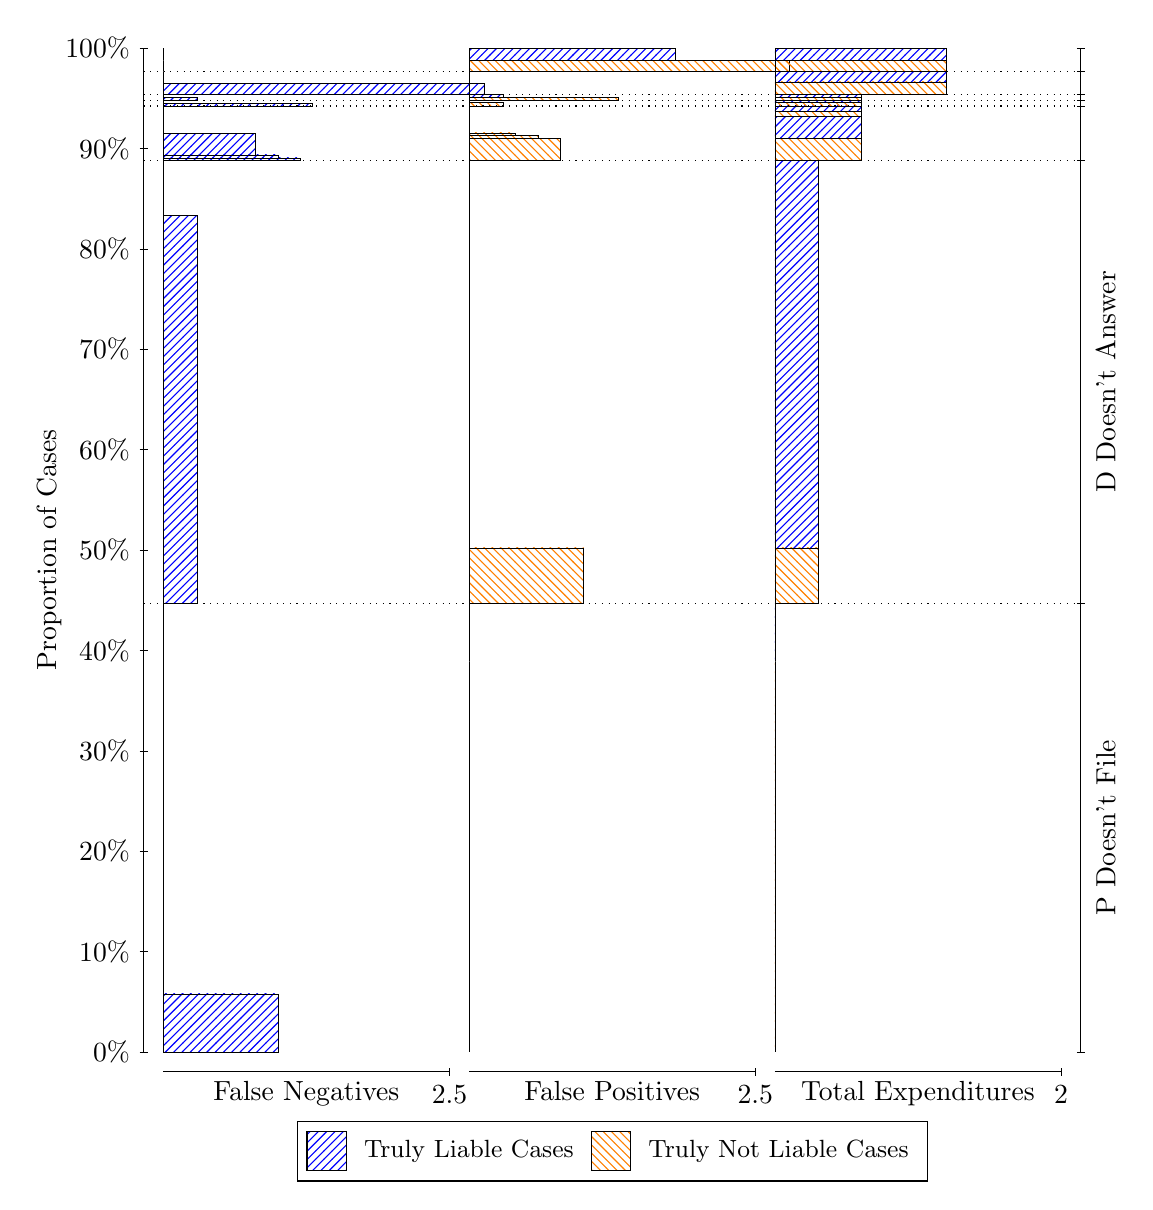
\begin{tikzpicture}
\draw[black, very thin] (1.5,1.75) -- (1.5,14.5);
\node[rotate=90, text=black, anchor=center] at (0.3, 8.125) {Proportion of Cases};
\draw[black, very thin] (1.45,1.75) -- (1.55,1.75);
\node[text=black, anchor=east] at (1.45, 1.75) {0\%};
\draw[black, very thin] (1.45,3.025) -- (1.55,3.025);
\node[text=black, anchor=east] at (1.45, 3.025) {10\%};
\draw[black, very thin] (1.45,4.3) -- (1.55,4.3);
\node[text=black, anchor=east] at (1.45, 4.3) {20\%};
\draw[black, very thin] (1.45,5.575) -- (1.55,5.575);
\node[text=black, anchor=east] at (1.45, 5.575) {30\%};
\draw[black, very thin] (1.45,6.85) -- (1.55,6.85);
\node[text=black, anchor=east] at (1.45, 6.85) {40\%};
\draw[black, very thin] (1.45,8.125) -- (1.55,8.125);
\node[text=black, anchor=east] at (1.45, 8.125) {50\%};
\draw[black, very thin] (1.45,9.4) -- (1.55,9.4);
\node[text=black, anchor=east] at (1.45, 9.4) {60\%};
\draw[black, very thin] (1.45,10.675) -- (1.55,10.675);
\node[text=black, anchor=east] at (1.45, 10.675) {70\%};
\draw[black, very thin] (1.45,11.95) -- (1.55,11.95);
\node[text=black, anchor=east] at (1.45, 11.95) {80\%};
\draw[black, very thin] (1.45,13.225) -- (1.55,13.225);
\node[text=black, anchor=east] at (1.45, 13.225) {90\%};
\draw[black, very thin] (1.45,14.5) -- (1.55,14.5);
\node[text=black, anchor=east] at (1.45, 14.5) {100\%};

\draw[black, very thin] (13.4,1.75) -- (13.4,14.5);
\draw[black, very thin] (13.35,1.75) -- (13.45,1.75);
\node[anchor=west] at (13.35, 1.75) {};
\draw[black, very thin] (13.35,7.4438) -- (13.45,7.4438);
\node[anchor=west] at (13.35, 7.4438) {};
\draw[black, very thin] (13.35,13.077) -- (13.45,13.077);
\node[anchor=west] at (13.35, 13.077) {};
\draw[black, very thin] (13.35,13.764) -- (13.45,13.764);
\node[anchor=west] at (13.35, 13.764) {};
\draw[black, very thin] (13.35,13.839) -- (13.45,13.839);
\node[anchor=west] at (13.35, 13.839) {};
\draw[black, very thin] (13.35,13.912) -- (13.45,13.912);
\node[anchor=west] at (13.35, 13.912) {};
\draw[black, very thin] (13.35,14.204) -- (13.45,14.204);
\node[anchor=west] at (13.35, 14.204) {};
\draw[black, very thin] (13.35,14.5) -- (13.45,14.5);
\node[anchor=west] at (13.35, 14.5) {};

\draw[black, very thin, pattern color=blue, pattern=north east lines] (1.75,1.75) rectangle (3.2033,2.4873);
\draw[black, very thin, pattern color=orange, pattern=north west lines] (1.75,2.4873) rectangle (1.75,7.4438);
\draw[black, very thin, pattern color=blue, pattern=north east lines] (1.75,7.4438) rectangle (2.186,12.37);
\draw[black, very thin, pattern color=orange, pattern=north west lines] (1.75,12.37) rectangle (1.75,13.077);
\draw[black, very thin, pattern color=blue, pattern=north east lines] (1.75,13.077) rectangle (3.494,13.104);
\draw[black, very thin, pattern color=blue, pattern=north east lines] (1.75,13.104) rectangle (3.2033,13.142);
\draw[black, very thin, pattern color=blue, pattern=north east lines] (1.75,13.142) rectangle (2.9127,13.42);
\draw[black, very thin, pattern color=orange, pattern=north west lines] (1.75,13.42) rectangle (1.75,13.764);
\draw[black, very thin, pattern color=blue, pattern=north east lines] (1.75,13.764) rectangle (3.6393,13.799);
\draw[black, very thin, pattern color=orange, pattern=north west lines] (1.75,13.799) rectangle (1.75,13.839);
\draw[black, very thin, pattern color=blue, pattern=north east lines] (1.75,13.839) rectangle (2.186,13.878);
\draw[black, very thin, pattern color=orange, pattern=north west lines] (1.75,13.878) rectangle (1.75,13.912);
\draw[black, very thin, pattern color=blue, pattern=north east lines] (1.75,13.912) rectangle (5.8193,14.047);
\draw[black, very thin, pattern color=orange, pattern=north west lines] (1.75,14.047) rectangle (1.75,14.204);
\draw[black, very thin, pattern color=orange, pattern=north west lines] (1.75,14.204) rectangle (1.75,14.34);
\draw[black, very thin, pattern color=blue, pattern=north east lines] (1.75,14.34) rectangle (1.75,14.5);
\draw[black, very thin, pattern color=orange, pattern=north west lines] (5.6333,1.75) rectangle (5.6333,6.7065);
\draw[black, very thin, pattern color=blue, pattern=north east lines] (5.6333,6.7065) rectangle (5.6333,7.4438);
\draw[black, very thin, pattern color=orange, pattern=north west lines] (5.6333,7.4438) rectangle (7.0867,8.1507);
\draw[black, very thin, pattern color=blue, pattern=north east lines] (5.6333,8.1507) rectangle (5.6333,13.077);
\draw[black, very thin, pattern color=orange, pattern=north west lines] (5.6333,13.077) rectangle (6.796,13.355);
\draw[black, very thin, pattern color=orange, pattern=north west lines] (5.6333,13.355) rectangle (6.5053,13.392);
\draw[black, very thin, pattern color=orange, pattern=north west lines] (5.6333,13.392) rectangle (6.2147,13.422);
\draw[black, very thin, pattern color=blue, pattern=north east lines] (5.6333,13.422) rectangle (5.6333,13.764);
\draw[black, very thin, pattern color=orange, pattern=north west lines] (5.6333,13.764) rectangle (6.0693,13.805);
\draw[black, very thin, pattern color=blue, pattern=north east lines] (5.6333,13.805) rectangle (5.6333,13.839);
\draw[black, very thin, pattern color=orange, pattern=north west lines] (5.6333,13.839) rectangle (7.5227,13.873);
\draw[black, very thin, pattern color=blue, pattern=north east lines] (5.6333,13.873) rectangle (6.0693,13.912);
\draw[black, very thin, pattern color=orange, pattern=north west lines] (5.6333,13.912) rectangle (5.6333,14.069);
\draw[black, very thin, pattern color=blue, pattern=north east lines] (5.6333,14.069) rectangle (5.6333,14.204);
\draw[black, very thin, pattern color=orange, pattern=north west lines] (5.6333,14.204) rectangle (9.7027,14.34);
\draw[black, very thin, pattern color=blue, pattern=north east lines] (5.6333,14.34) rectangle (8.2493,14.5);
\draw[black, very thin, pattern color=orange, pattern=north west lines] (9.5167,1.75) rectangle (9.5167,6.7065);
\draw[black, very thin, pattern color=blue, pattern=north east lines] (9.5167,6.7065) rectangle (9.5167,7.4438);
\draw[black, very thin, pattern color=orange, pattern=north west lines] (9.5167,7.4438) rectangle (10.062,8.1507);
\draw[black, very thin, pattern color=blue, pattern=north east lines] (9.5167,8.1507) rectangle (10.062,13.077);
\draw[black, very thin, pattern color=orange, pattern=north west lines] (9.5167,13.077) rectangle (10.607,13.355);
\draw[black, very thin, pattern color=blue, pattern=north east lines] (9.5167,13.355) rectangle (10.607,13.632);
\draw[black, very thin, pattern color=orange, pattern=north west lines] (9.5167,13.632) rectangle (10.607,13.699);
\draw[black, very thin, pattern color=blue, pattern=north east lines] (9.5167,13.699) rectangle (10.607,13.764);
\draw[black, very thin, pattern color=orange, pattern=north west lines] (9.5167,13.764) rectangle (10.607,13.805);
\draw[black, very thin, pattern color=blue, pattern=north east lines] (9.5167,13.805) rectangle (10.607,13.839);
\draw[black, very thin, pattern color=orange, pattern=north west lines] (9.5167,13.839) rectangle (10.607,13.873);
\draw[black, very thin, pattern color=blue, pattern=north east lines] (9.5167,13.873) rectangle (10.607,13.912);
\draw[black, very thin, pattern color=orange, pattern=north west lines] (9.5167,13.912) rectangle (11.697,14.069);
\draw[black, very thin, pattern color=blue, pattern=north east lines] (9.5167,14.069) rectangle (11.697,14.204);
\draw[black, very thin, pattern color=orange, pattern=north west lines] (9.5167,14.204) rectangle (11.697,14.34);
\draw[black, very thin, pattern color=blue, pattern=north east lines] (9.5167,14.34) rectangle (11.697,14.5);
\draw[black, dotted] (1.5,7.4438) -- (13.4,7.4438);
\draw[black, dotted] (1.5,13.077) -- (13.4,13.077);
\draw[black, dotted] (1.5,13.764) -- (13.4,13.764);
\draw[black, dotted] (1.5,13.839) -- (13.4,13.839);
\draw[black, dotted] (1.5,13.912) -- (13.4,13.912);
\draw[black, dotted] (1.5,14.204) -- (13.4,14.204);
\draw[black, very thin] (1.75,1.5) -- (5.3833,1.5);
\node[text=black, anchor=north] at (3.5667, 1.5) {False Negatives};
\draw[black, very thin] (5.3833,1.45) -- (5.3833,1.55);
\node[text=black, anchor=north] at (5.3833, 1.45) {2.5};

\draw[black, very thin] (5.6333,1.5) -- (9.2667,1.5);
\node[text=black, anchor=north] at (7.45, 1.5) {False Positives};
\draw[black, very thin] (9.2667,1.45) -- (9.2667,1.55);
\node[text=black, anchor=north] at (9.2667, 1.45) {2.5};

\draw[black, very thin] (9.5167,1.5) -- (13.15,1.5);
\node[text=black, anchor=north] at (11.333, 1.5) {Total Expenditures};
\draw[black, very thin] (13.15,1.45) -- (13.15,1.55);
\node[text=black, anchor=north] at (13.15, 1.45) {2};

\node[text=black, centered, rotate=90] at (13.72, 4.5969) {P Doesn't File};
\node[text=black, centered, rotate=90] at (13.72, 10.26) {D Doesn't Answer};






\draw (7.449999999999999,1.5) node[draw=none] (baseCoordinate) {};
\begin{scope}[align=center]
        \matrix[scale=0.5, draw=black, below=0.5cm of baseCoordinate, nodes={draw}, column sep=0.1cm]{
            \node[rectangle, draw, minimum width=0.5cm, minimum height=0.5cm, pattern color=blue, pattern=north east lines] {}; &
            \node[draw=none, font=\small, text=black] (B) {Truly Liable Cases}; &
            \node[rectangle, draw, minimum width=0.5cm, minimum height=0.5cm, pattern color=orange, pattern=north west lines] {}; &
            \node[draw=none, font=\small, text=black] (B) {Truly Not Liable Cases}; \\
            };
\end{scope}

\end{tikzpicture}
\end{document}